\documentclass[./project-report/src/latex/project-report.tex]{subfiles}

\begin{document}

\maketitle

\section{Testing TODO}

\subsection{Investigation}

\subsubsection{test\_model module}

The test\_model module is contained within the frames package, and contains tkinter frames for testing the trained Artificial Neural Network models for each dataset. 
Each frame displays the results of the testing along with a random selection of incorrect and correct predictions.

\inputminted{python}{./school_project/frames/test_model.py}

Which outputs the following for the MNIST dataset:

\pagebreak

\begin{figure}[h!]
\centering
\frame{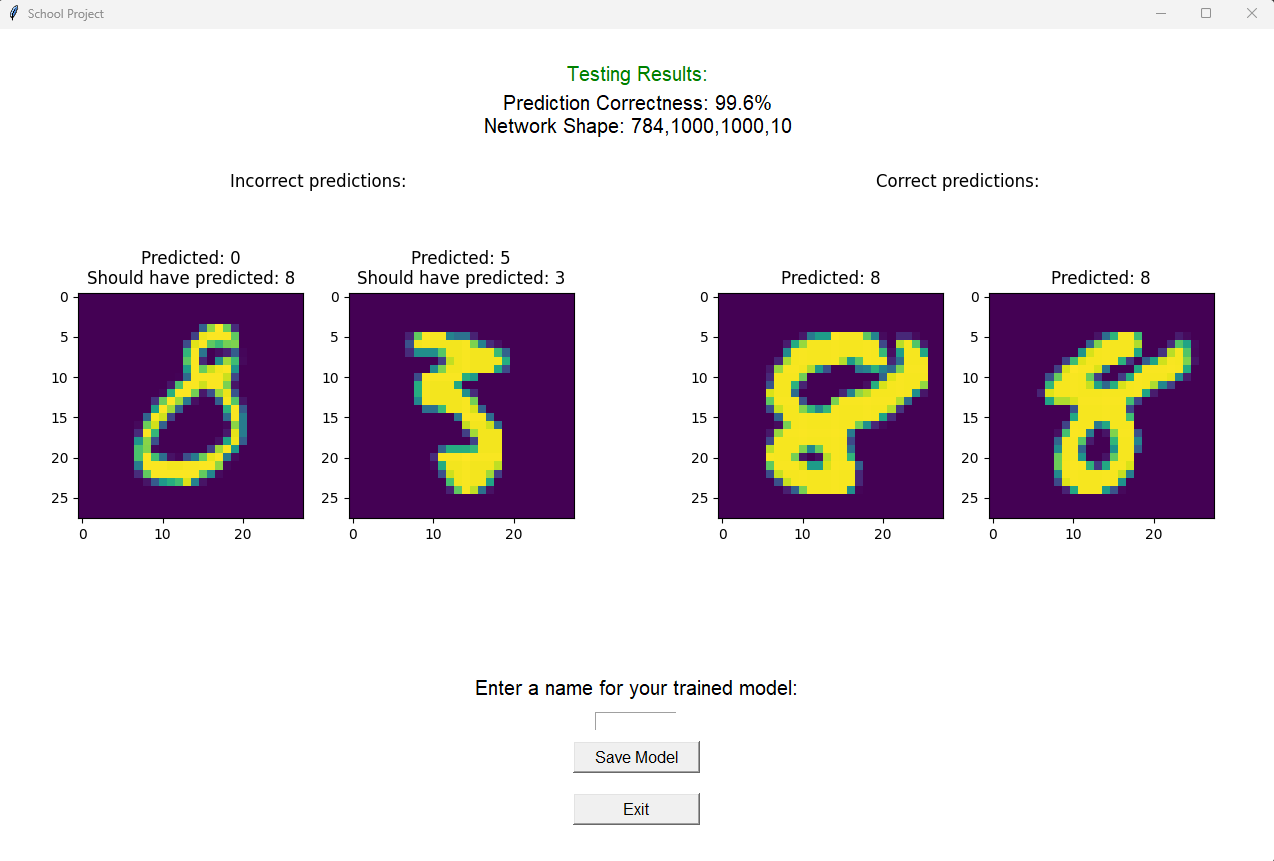
\includegraphics[width=1\textwidth]{./project-report/src/images/test-mnist-frame.png}}
\end{figure}

And outputs the following for the Cat Recognition dataset:

\pagebreak

\begin{figure}[h!]
\centering
\frame{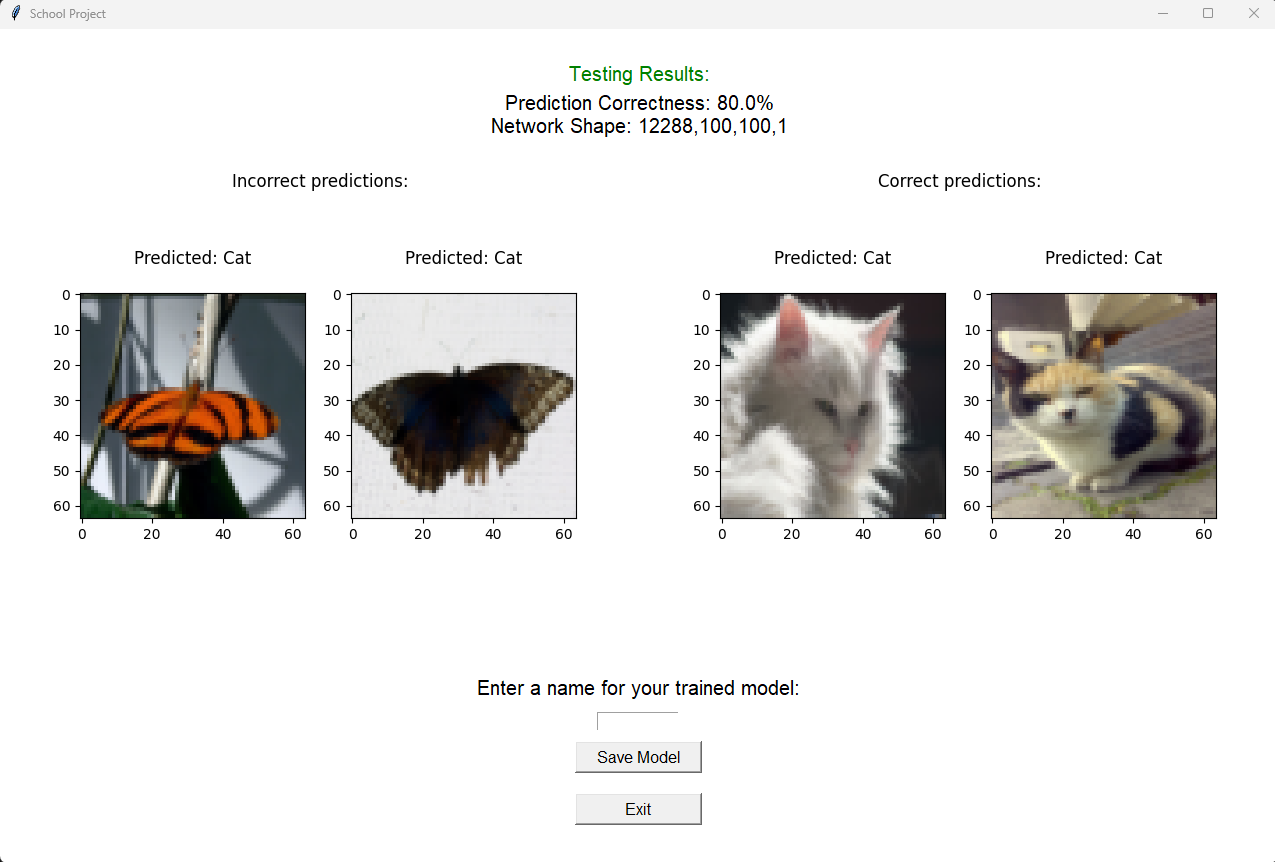
\includegraphics[width=1\textwidth]{./project-report/src/images/test-cat-recognition-frame.png}}
\end{figure}

And outputs the following for the XOR dataset:

\pagebreak

\begin{figure}[h!]
\centering
\frame{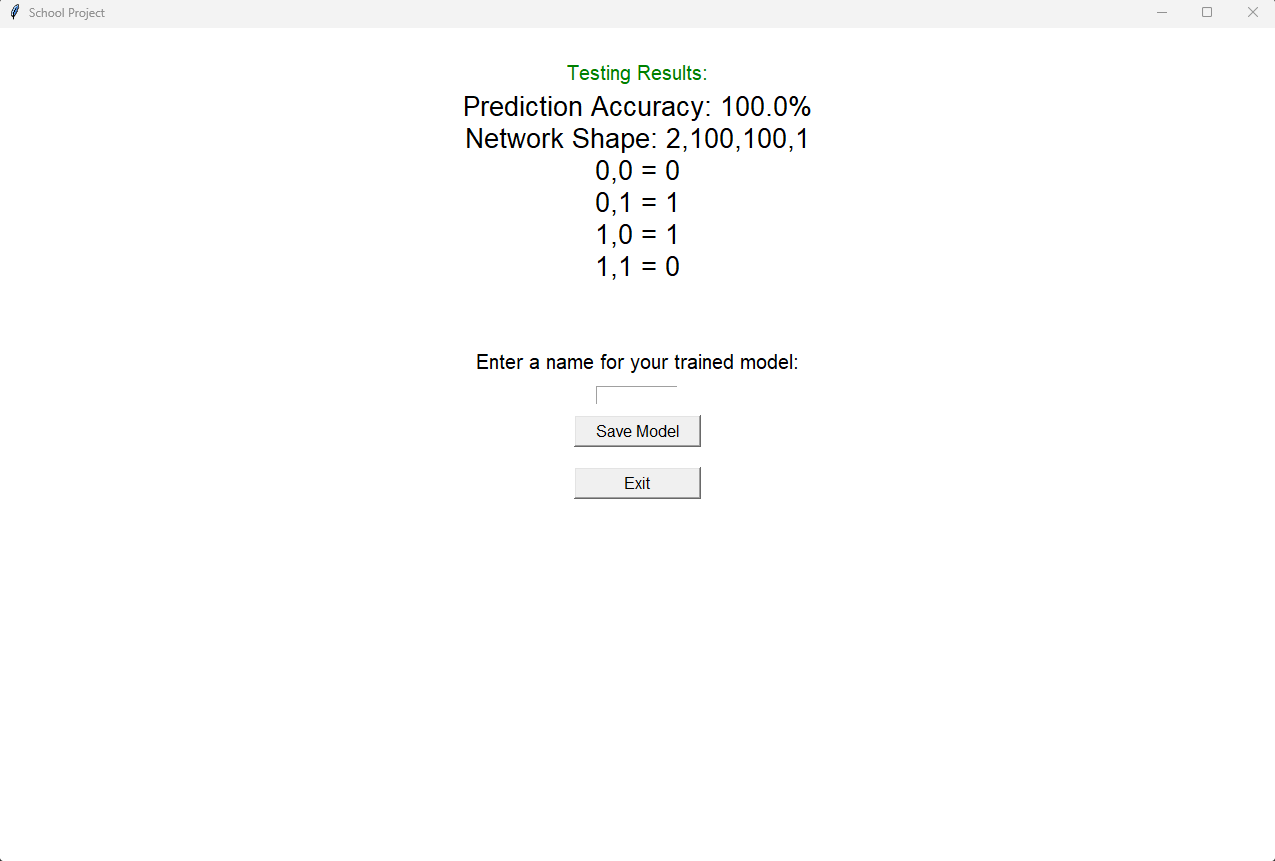
\includegraphics[width=1\textwidth]{./project-report/src/images/test-xor-frame.png}}
\end{figure}

\subsubsection{Effects of Hyper-Parameters}

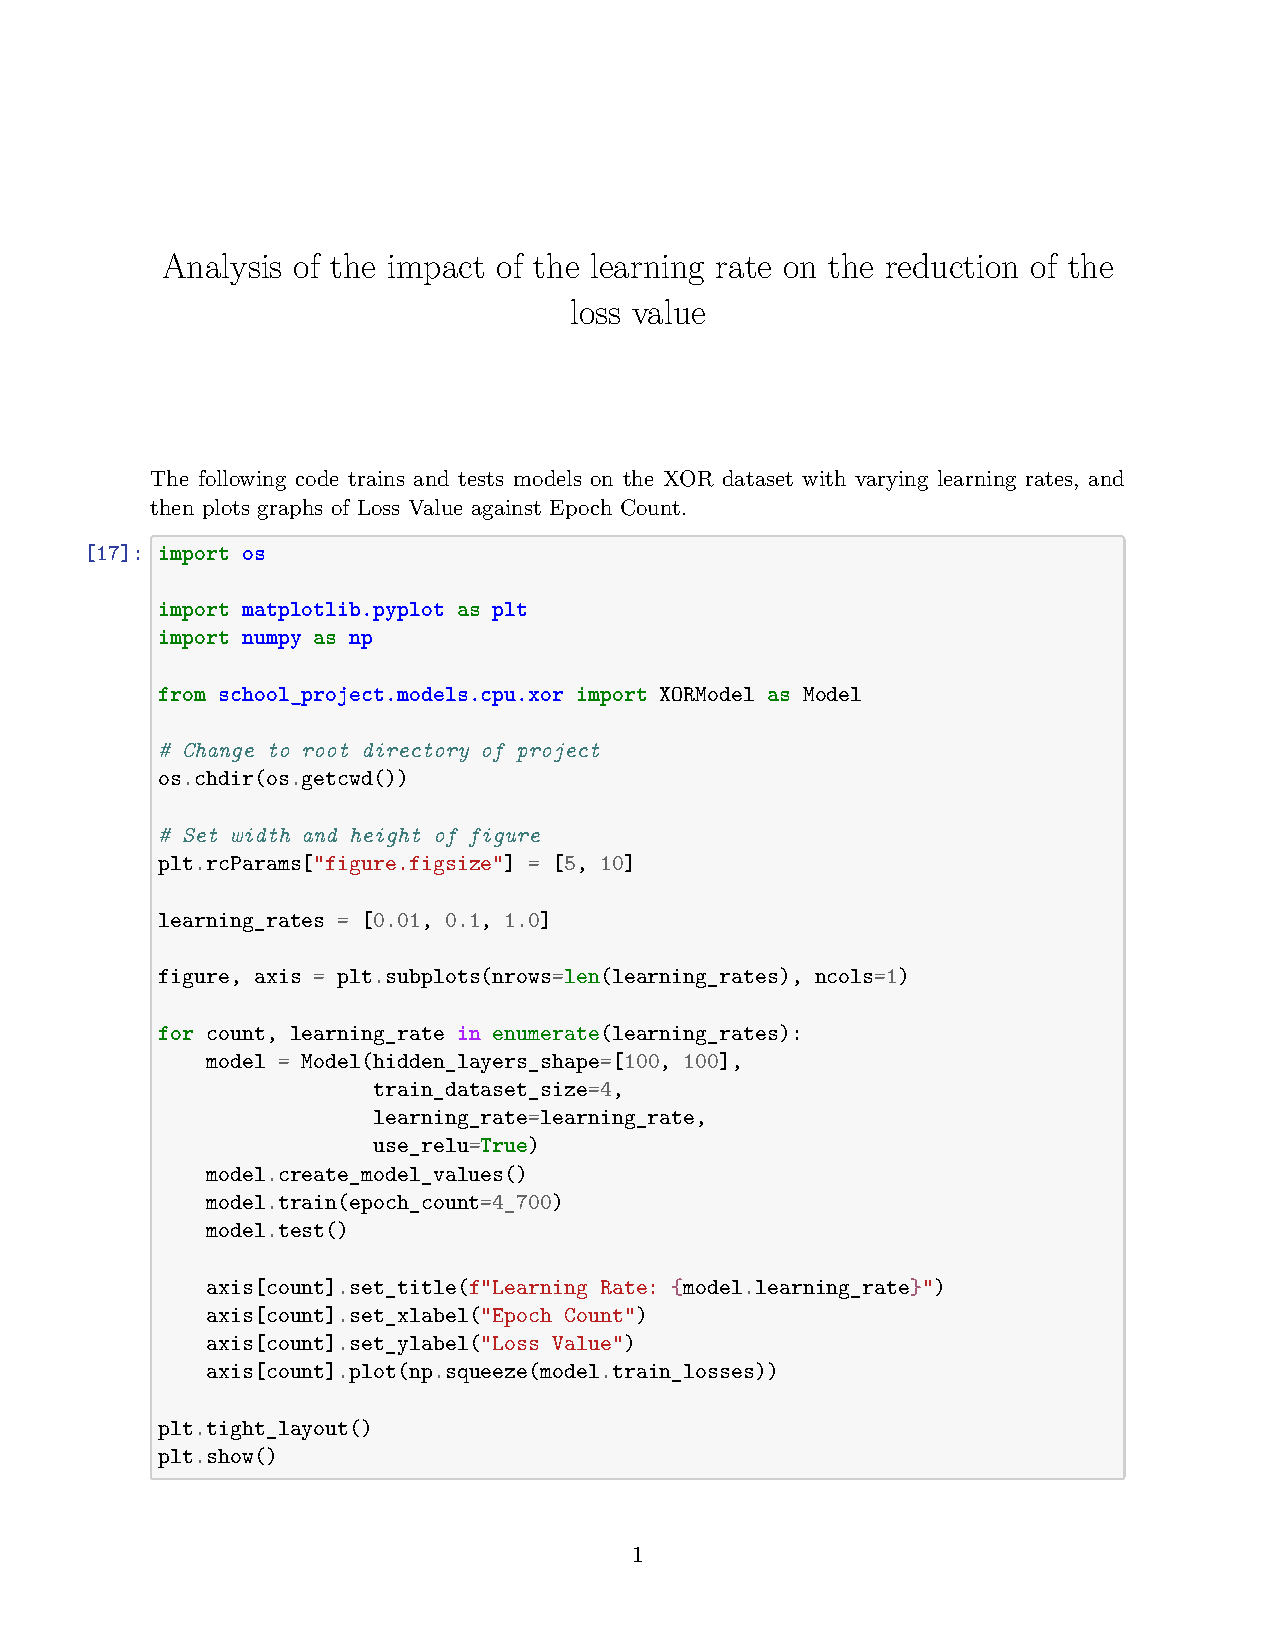
\includepdf[pages=-, pagecommand={\thispagestyle{plain}}, scale=0.9]{./project-report/src/pdfs/learning-rate-analysis.pdf}
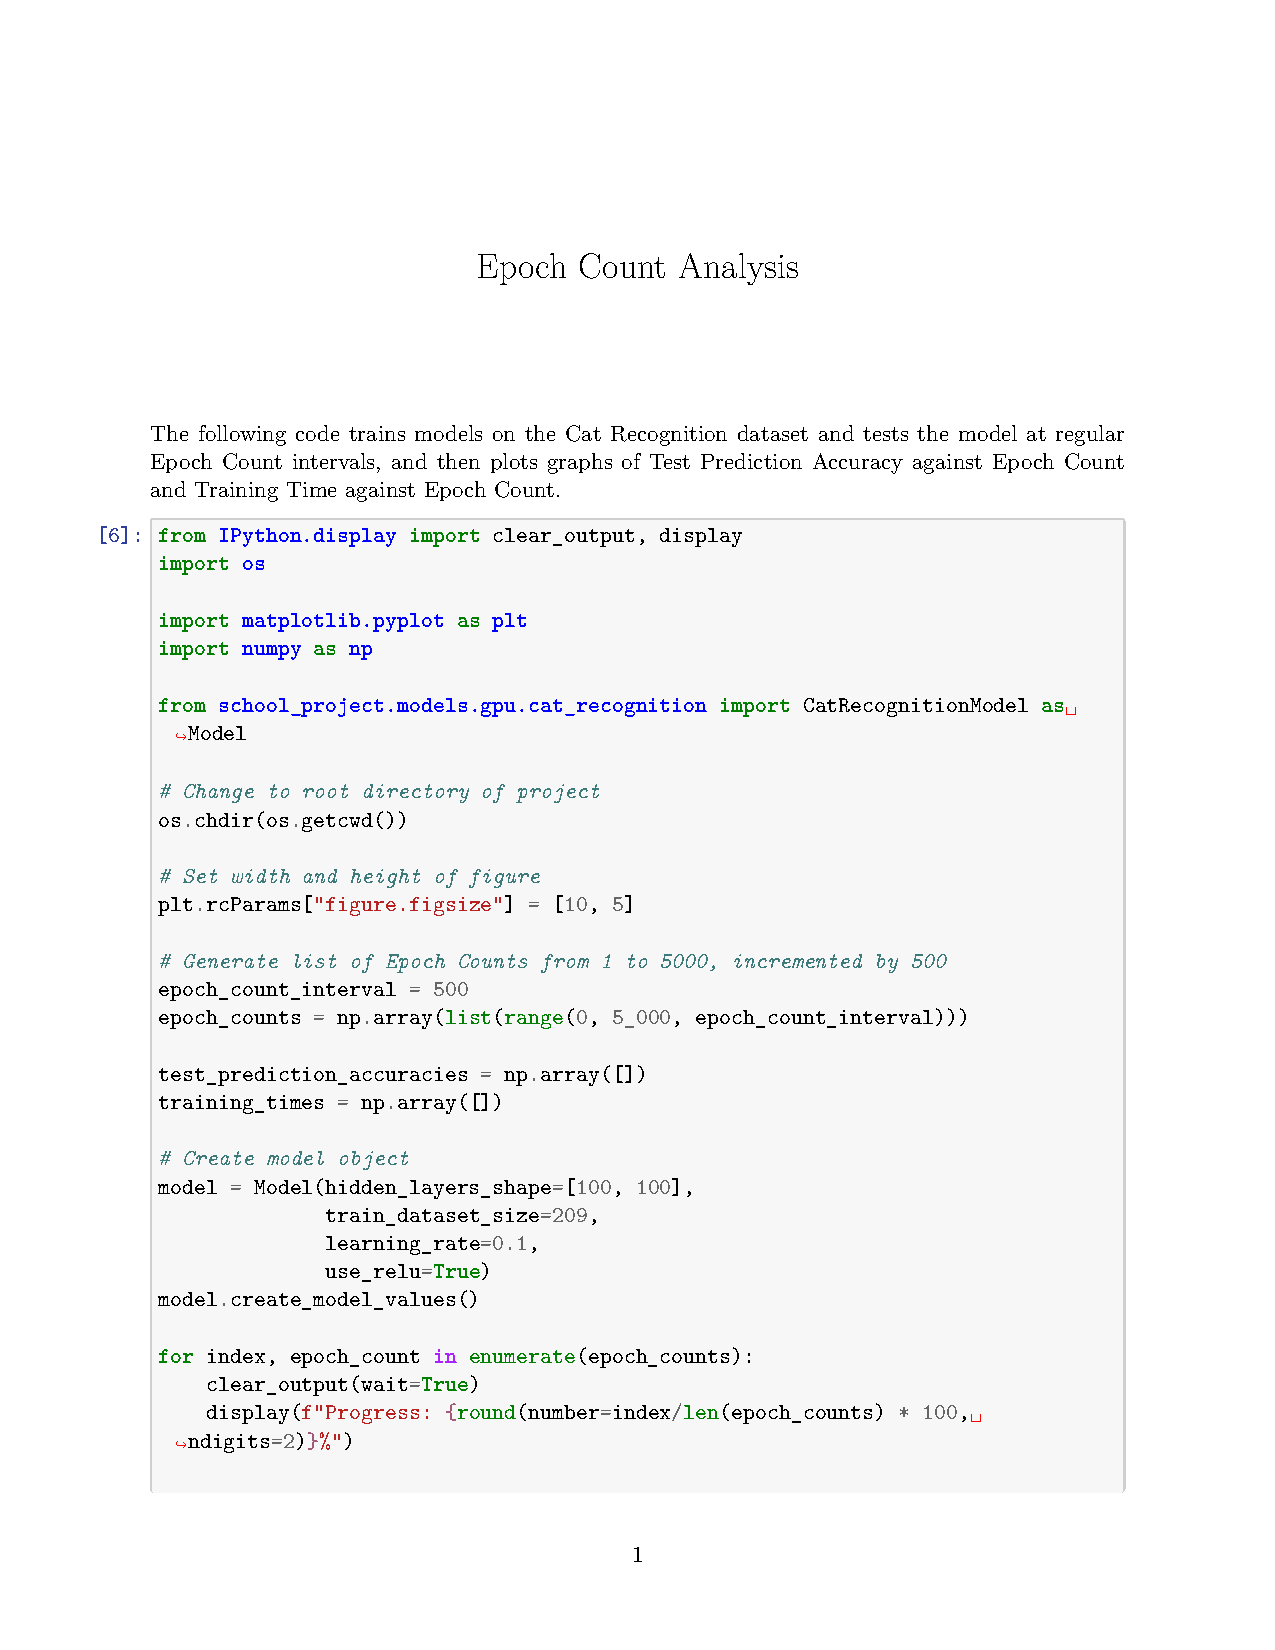
\includepdf[pages=-, pagecommand={\thispagestyle{plain}}, scale=0.9]{./project-report/src/pdfs/epoch-count-analysis.pdf}
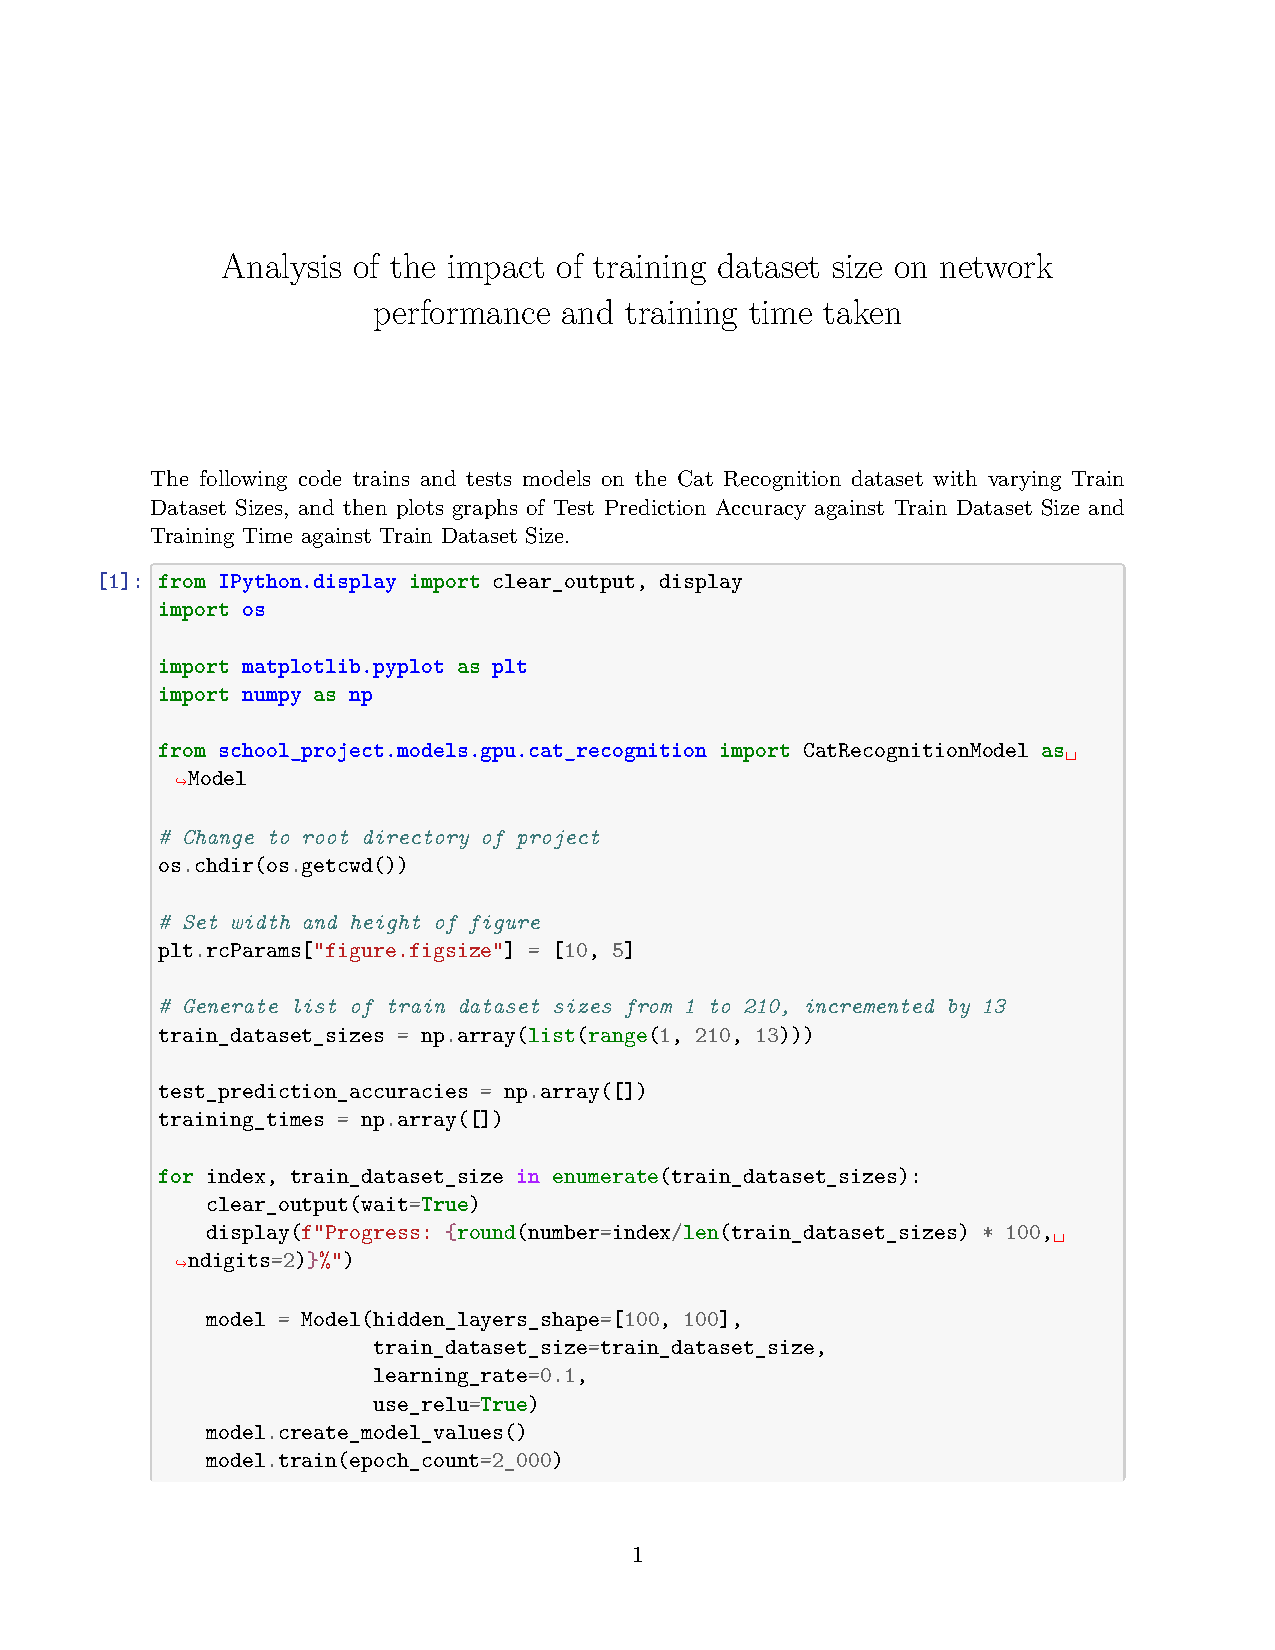
\includepdf[pages=-, pagecommand={\thispagestyle{plain}}, scale=0.9]{./project-report/src/pdfs/train-dataset-size-analysis.pdf}
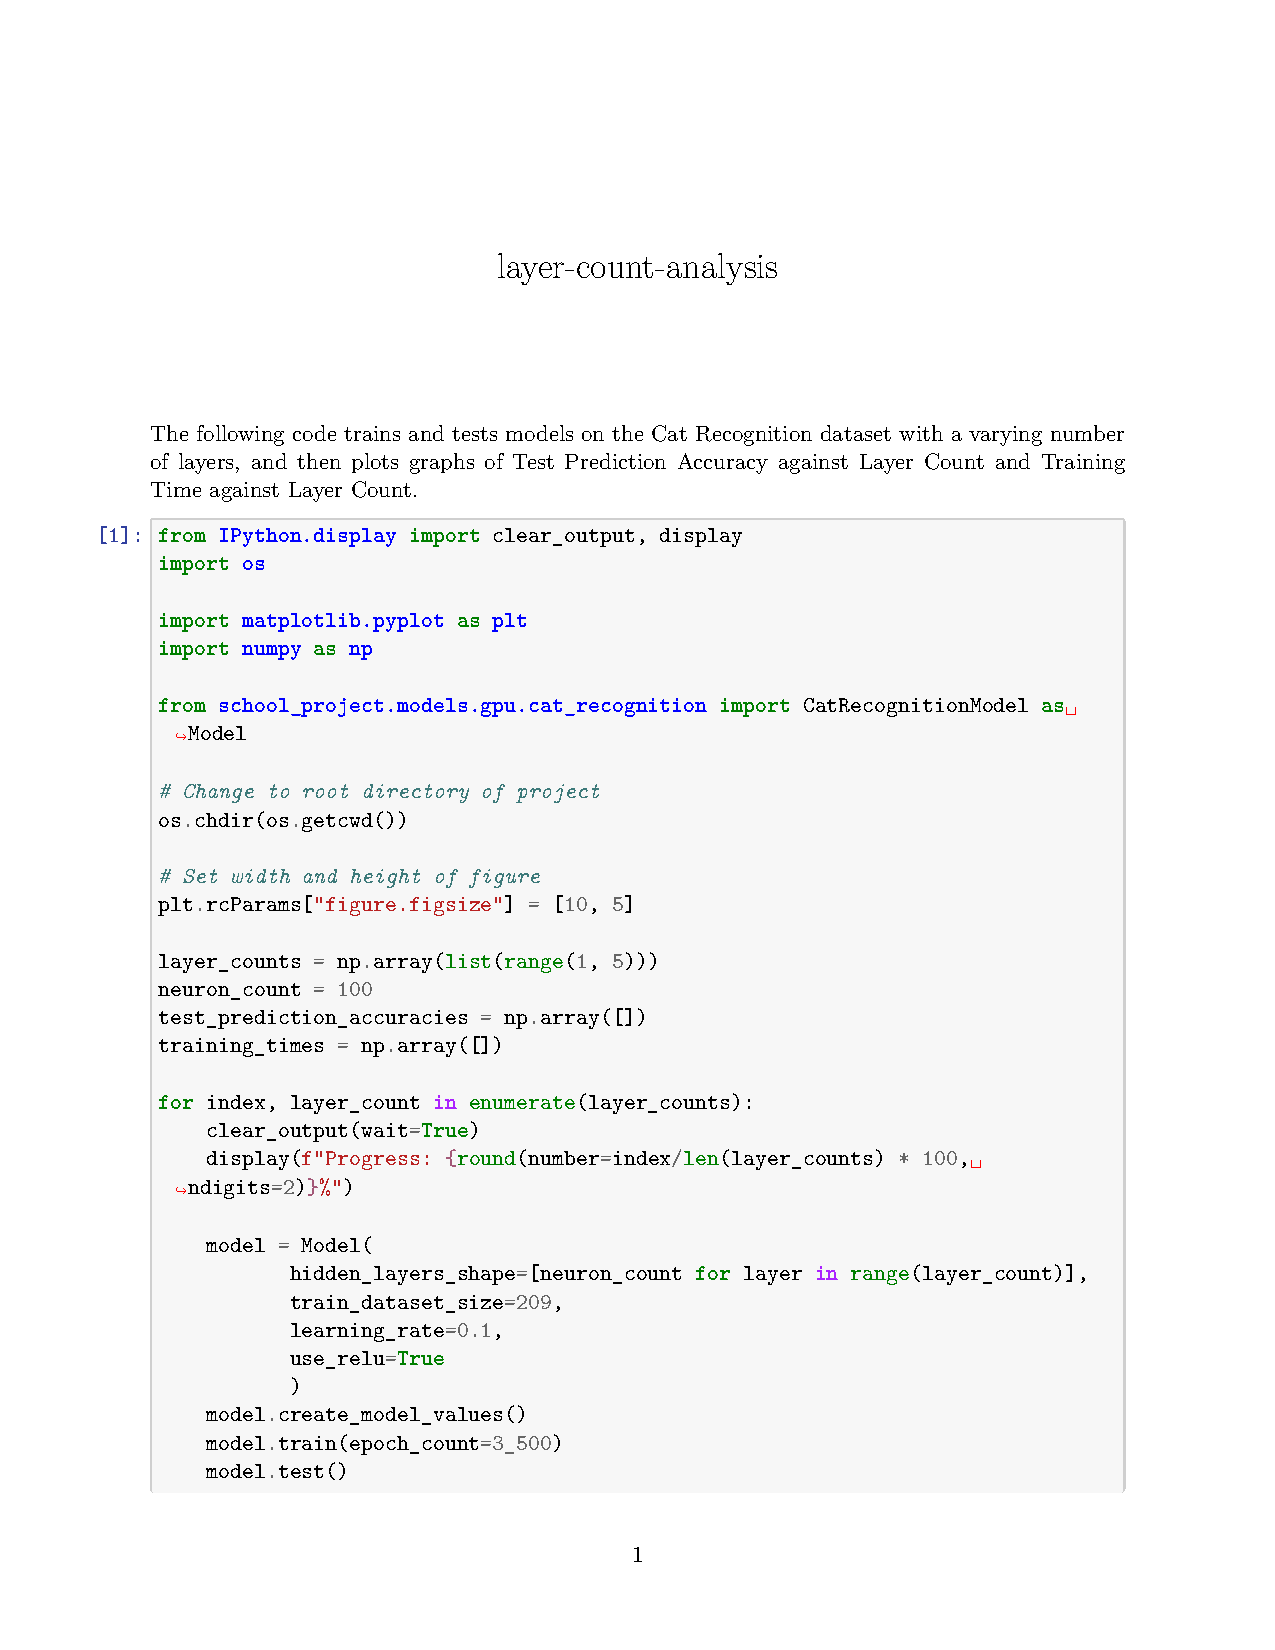
\includepdf[pages=-, pagecommand={\thispagestyle{plain}}, scale=0.9]{./project-report/src/pdfs/layer-count-analysis.pdf}
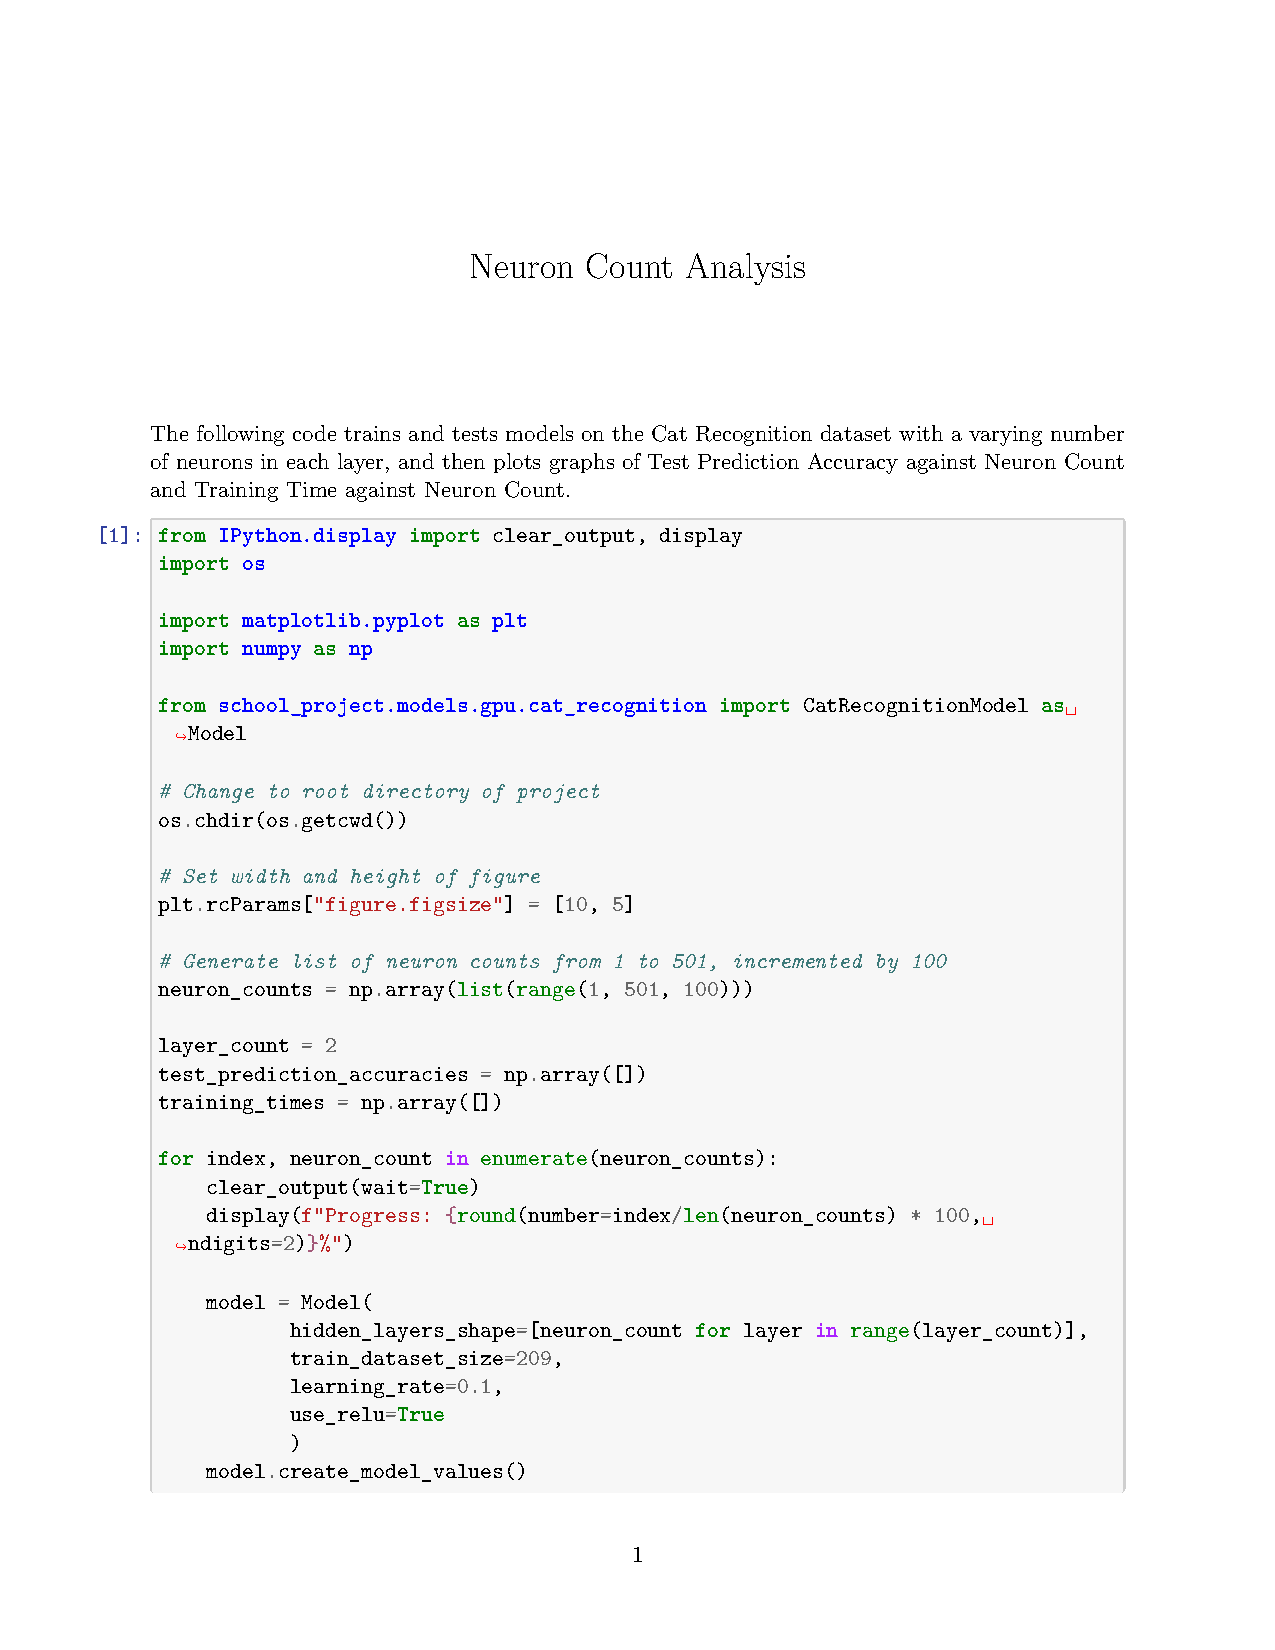
\includepdf[pages=-, pagecommand={\thispagestyle{plain}}, scale=0.9]{./project-report/src/pdfs/neuron-count-analysis.pdf}
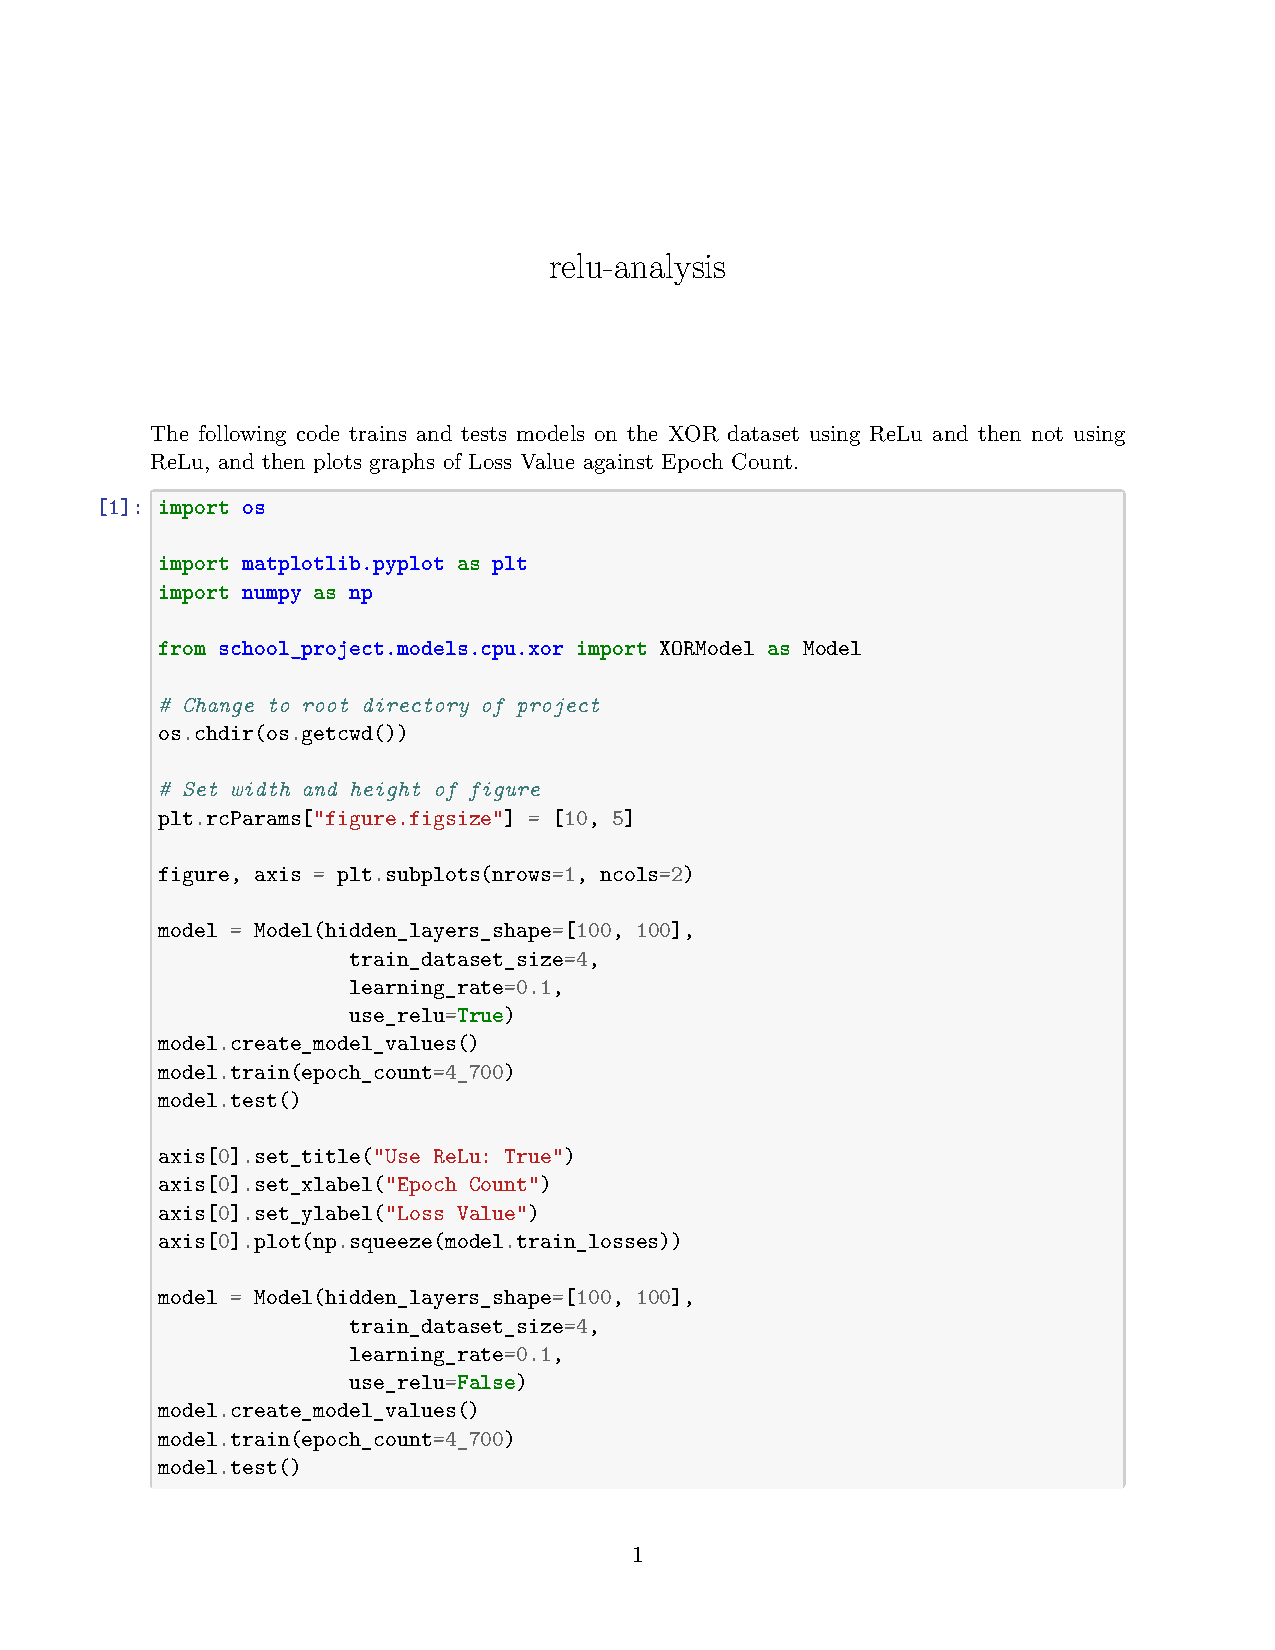
\includepdf[pages=-, pagecommand={\thispagestyle{plain}}, scale=0.9]{./project-report/src/pdfs/relu-analysis.pdf}
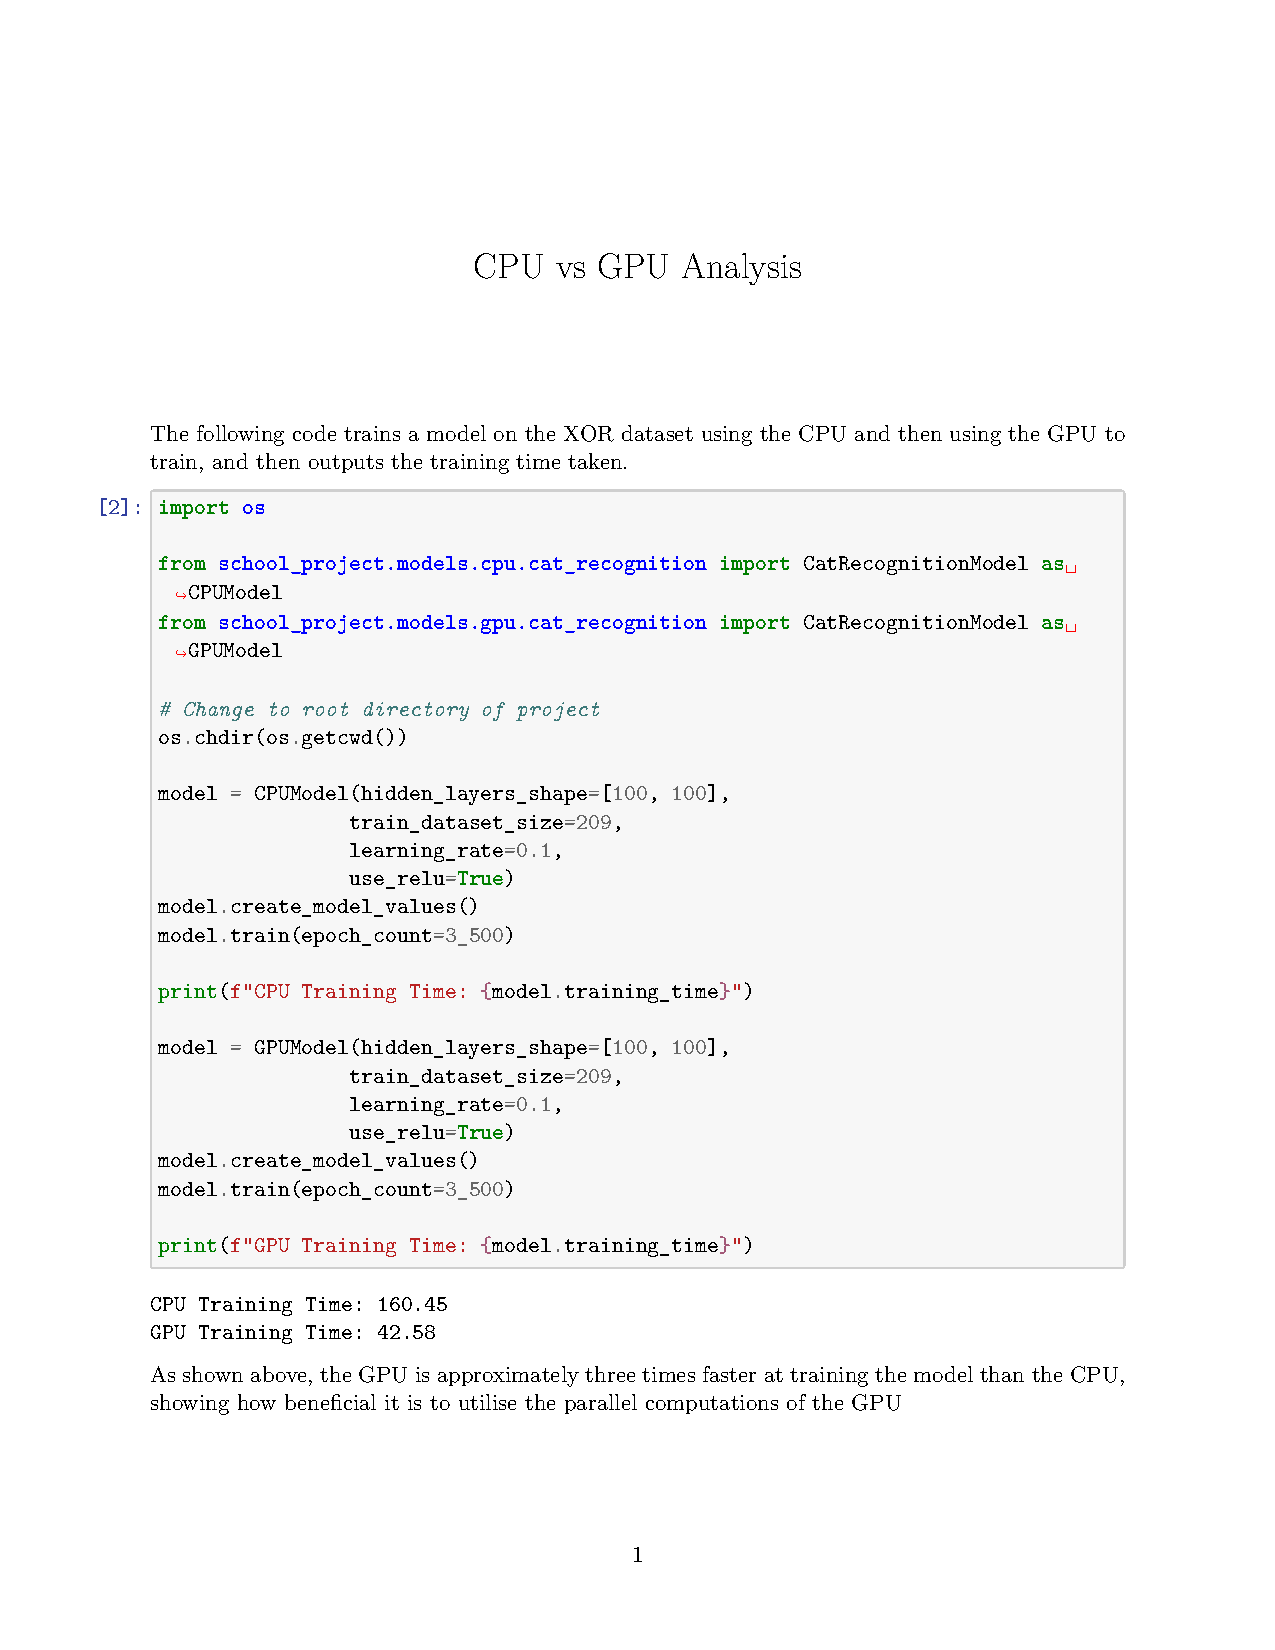
\includepdf[pages=-, pagecommand={\thispagestyle{plain}}, scale=0.9]{./project-report/src/pdfs/cpu-vs-gpu-analysis.pdf}

\subsection{Manual Testing}

\subsubsection{Input Validation Testing TODO}  % Add input validation images in table

\subsection{Automated Testing}

\subsubsection{Unit Tests}

Within the test package, I have written the following unit tests for the utils subpackage of both the cpu and gpu subpackage of the models package. Similarly to the code for the cpu 
and gpu subpackage, it is only worth showing the code for the cpu version as both are very similar in functionality.

\begin{itemize}
    \item test\_model.py module:
        \inputminted{python}{./school_project/test/models/cpu/utils/test_model.py}

        \pagebreak

    \item test\_tools.py module:
        \inputminted{python}{./school_project/test/models/cpu/utils/test_tools.py}
\end{itemize}

\inputminted{python}{./school_project/test/models/cpu.py}

\subsubsection{GitHub Automated Testing}

With the following configuration programmed in the .github/workflows/tests.yml file, the unit tests are run automatically on GitHub servers after each commit that is pushed to GitHub, 
and the status of the tests (either passing or failing) can be viewed on the repository's page. This automatic testing allows for a faster workflow and allows me to identify which changes 
(commits) cause issues within the code, allowing for easier maintenance of the project.

\inputminted{yaml}{./.github/workflows/tests.yml}

\end{document}